\documentclass[a4paper]{article}

\usepackage[utf8]{inputenc}
\usepackage[ngerman]{babel}
\usepackage{amsmath,amssymb}
\usepackage[german,vlined,longend]{algorithm2e}
\usepackage{graphicx}
\PassOptionsToPackage{usenames,dvipsnames,svgnames}{xcolor}  
\usepackage{tikz}
\usetikzlibrary{arrows,positioning,automata}
\usepackage{listings}

% --- math operators ---
\usepackage{mathtools}
\DeclarePairedDelimiter\set{\{}{\}} % use $\set*{1, 2, 3}$ 
\DeclarePairedDelimiter\abs{\lvert}{\rvert}
\DeclarePairedDelimiter\norm{\lVert}{\rVert}
\DeclarePairedDelimiter\ceils{\lceil}{\rceil}
\DeclarePairedDelimiter\floor{\lfloor}{\rfloor}
\DeclarePairedDelimiter\angles{\langle}{\rangle}
\def\Oh{\ensuremath{\mathcal{O}}} % big O like $\Oh(n)$
\def\oh{\ensuremath{\scriptstyle{\mathcal{O}}}} % small O
% ---

\begin{document}

\begin{small}
	\noindent
	Schubert Julian, Gruppe 4 \\
	Philipp Wahl, Gruppe 4
\end{small}
\bigskip

\begin{center}
	\LARGE Abgabe zum 2. Übungsblatt (AGT 21)
\end{center}
\smallskip

\subsection*{Aufgabe 1:}

\paragraph{a)}
\begin{tabular}{ |c | c | c | c | c | c | c |}
    \hline
    \textbf{t}  & \textbf{u}& \textbf{v}& \textbf{w}& \textbf{x}& \textbf{y}& \textbf{z} \\
    \hline
    $\infty$    & $\infty$  & $\infty$  & $\infty$  & 0         & $\infty$  & $\infty$ \\
    $\infty$    & \textbf{2}& 3         & 6         & 0         & $\infty$  & $\infty$ \\
    $\infty$    &           &\textbf{3} & 6         & 0         & 12        & $\infty$ \\
    $\infty$    &           &           & \textbf{5}& 0         & 12        & 9 \\
    9           &           &           &           & 0         & 12        &\textbf{7} \\
    \textbf{9}  &           &           &           & 0         & 10        & \\
                &           &           &           & 0         & \textbf{10}& \\
    \hline
\end{tabular}
\paragraph{b)}
Die erste Abbildung zeigt ein Beispiel bei dem der Algorithmus von Dijkstra fehl schlägt. Startet 
man hier vom Knoten q0 bekommt im nächsten Schritt der Knoten q1 eine Distanz von 1 zugeteilt.
Jedoch sind die tatsächlichen Kosten des Pfades zu q1 minus unendlich da die Katne von q1 nach 
q2 ein Gewicht von minus 4 hat, man also immer weiter im Kreis gehen kann und der Weg immer
billiger wird. \\
\begin{figure}[htb]
\centering
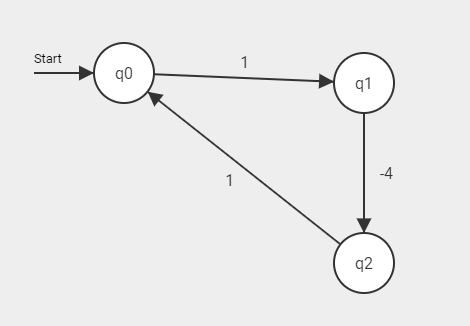
\includegraphics[width=0.9\linewidth]{01.png}
\label{dijkstrabad}
\caption{Hier schlägt Dijkstra fehl}
\end{figure}
Die zweite Abbildung zeigt ein Beispiel in dem der Algorighmus von Dijkstra funktioniert. Hier 
funktioniert der Algorithmus da nur ein einziges Mal eine negative Kante benutzt werden kann, und 
zwar die Kante die vom Start-Knoten 5 zum Knoten 1 führt
\begin{figure}[htb]
\centering
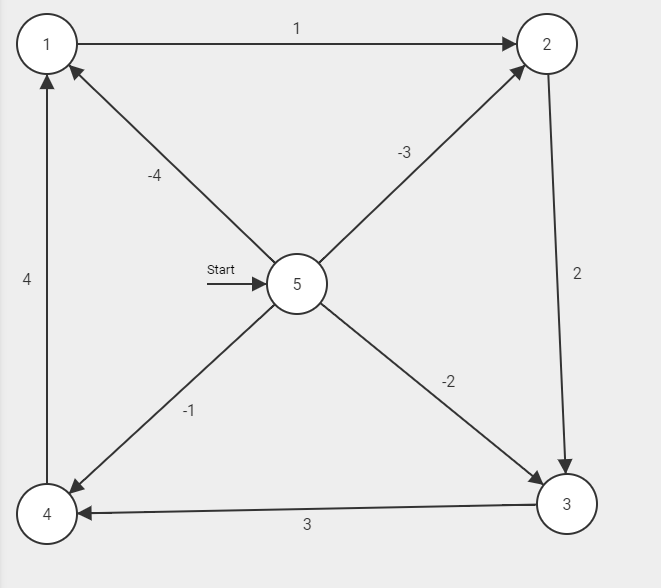
\includegraphics[width=0.9\linewidth]{02.png}
\caption{Hier funktioniert Dijkstra}
\label{fig:dijkstra_good}
\end{figure}

\section{Aufagbe 2}

\paragraph{a)}
\noindent HatKreis($G$, start)\\
\begin{algorithm}[H]
    // Speichert alle schon besuchten Knoten in Reihenfolge \\
    besucht = [] \\
    besucht.append(start) \\
    counter = 0 \\
    \While(Wir besuchen jeden Knoten maximal ein mal)
    {besucht.length != $|V|$ and counter != -1}{
        // Nimm den ersten Knoten aus der Adjazenzliste vom 
        aktuellen Knoten \\
        adj = besucht[counter].adj[0] \\
        \If(Zurück zum letzten Knoten gehen)
        {adj == nil}{
            counter -=1 \\
            continue \\
        }
        // Entferne den Knoten von eben aus der Adjazenzliste
        damit er nicht nocheinmal besucht wird \\
        vistited[counter].adj.remove(adj) \\

        \If(Wenn wir auf einem Knoten gelandet sind den 
        wir schonmal besucht haben existiert ein Kreis){adj.schonGesehen == true}{
            \Return true \\
        }

        // Speichern das wir den aktuellen Knoten schon 
        besucht haben \\
        ajd.schonGesehen = true \\

        // Zum nächsten Knoten gehen \\
        counter += 1 \\
        visited.append(adj)

    }
    // Es wurde kein Kreis gefunden \\
    \Return false \\
\end{algorithm}
Die Idee des Algorithmus ist die folgende: \\
Man speichert jeden schonmal besuchten Knoten in eine Liste, das sorgt dafür, dass 
die While-Schleife maximal $|V|$-mal läuft. Wir wählen dann den ersten Knoten in der 
Adjazenzliste des aktuellen Knotens aus. Wenn dieser Knoten nicht existiert gehen wir 
zurück, besuchen also den vorletzen besuchten Knoten. Dann entfernen wir den gerade 
Besuchten Knoten aus der Adjazenzliste. Haben wir den Knoten schon einmal gesehen so sind 
wir im Kreis gelaufen, es existiert also ein Kreis. Sonst markieren wir den 
Knoten als bereits gesehen und gehen dann zum nächsten Knoten (welches wieder 
der erste Knoten aus der Adjazenzliste des aktuellen Knotens ist)
\paragraph{b)}
\textbf{Laufzeit:} Da wir jeden noch nicht besuchten Knoten sofort zu der Liste 
Hinzufügen wird die While-Schleife maximal $|V|$-mal ausgeführt. \\
\textbf{Korrektheit:} Da wir jeden Knoten besuchen und abspeichern ob der Knoten
zuvor schon besucht wurde ist der Algorithmus korrekt.
\paragraph{c)}
Wenn unser counter auf -1 fällt bedeutet das im Algorithmus von oben das 
wir keinen Knoten mehr haben von dem wir aus weiter gehen könnten. 
Im nicht zusammenhängenden Graphen könnten wir eine zweite Liste einführen, 
in der zunächst alle Knoten gespeichert sind (also eine Kopie von $|V$). Wird 
ein Knoten zu besucht hinzugefügt wird er aus der zweiten Liste entfernt. 
Wenn dann counter gleich -1 ist (es also von allen besuchten Knoten aus
keinen weg mehr gibt den man gehen kann) wählen wir einen zufälligen Knoten
aus der zweiten Liste aus (da diese Liste alle Knoten enthält die wir noch 
nicht besucht haben) und führen den Algorithmus von dort fort. Das stellt 
sicher das wir auch im nicht zusammenhängenden Graphen alle Knoten besuchen 
und somit alle Kreise finden.
\section{Aufgabe 3}
\paragraph{a)}
CompleteHamilton wählt (beginnend am Startknoten s) und fügt den Knoten mit 
billgster Distanz zu C hinzu. Prim wählt ebenfalls zunächst den Startknoten, 
da dieser mit Distanz 0 initialisert wird. \\
In der While-Schleife wählen wir in Complete-Hamilton den Knoten aus, der 
am nähesten an C dran ist und fügen diesen zu C hinzu. Prim fügt ebenfalls 
den Knoten der am nähesten an den bereits behandelten Knoten ist hinzu.
Dies ist gegeben da wir in Relax alle Distanzen zu den jeweilig infrage 
kommenden Knoten updaten, und mit u = Q.ExtractMin() dann eben genau 
den Knoten wählen, der noch nicht besucht wurde und die geringste 
Distanz zu den bereits besuchten Knoten hat.
\paragraph{b)}
Um aus einem minimalen Spannbaum eine 2-Approximation für TSP zu 
erhalten werden zunächst alle Kanten verdoppelt, bereits besuchte 
Knoten übersprungen und dann eine Abkürzung eingefügt. Der Algorithmus
completeHamilton erstellt bereits den Graphen mit den Abkürzungen, er
erstellt also einen Hamiltonpfad. Um aus dem Pfad einen Kreis zu machen
müssen nun nur noch Start und Endknoten verbunden werden. Da der Graph
vollständig ist existiert eine solche direkte Kante. Durch die 
Dreiecksungleichung ist diese Kante sogar optimal (es gibt keinen
Kürzeren Weg vom Startknoten zum Endknoten). 
\end{document}